\scanpage{63}
$L(t)$ une fonction rat. en $t$, \deleted{\unsure{poids}} $q=p^{\unsure{f}}$
\[
L\left(\frac1{qt}\right)=A(t)L(t)\qquad A(t)\text{ de ``niveau'' inférieur}
\]
On veut simplifier l'équation fonctionnelle, en posant
\[
L'(t)=\lambda(t)L(t)
\]
d'où
\[
\begin{aligned}
L'\left(\frac1{qt}\right)&=\lambda\left(\frac1{qt}\right)L\left(\frac1{qt}\right)=\lambda\left(\frac1{qt}\right)A(t)L(t)\\
&=\lambda\left(\frac1{qt}\right)\lambda(t)^{-1}A(t)L'(t)
\end{aligned}
\]
et on aimerait obtenir $L'(\frac1{qt})=cL'(t)$, i.e.
\[
\frac{\lambda(\frac1{qt})}{\lambda(t)}=cA(t)^{-1}
\]
Si on trouve un tel $\lambda$, tout autre $\lambda'(t)=\alpha(t)\lambda(t)$ \inserted{avec une $\unsure{c^{te}}$ $c'$} est déterminé par $\alpha$ satisfaisant
\[
\frac{\alpha(\frac1{qt})}{\alpha(t)}=\frac{c'}c\qquad\text{i.e.}\quad\alpha\left(\frac1{qt}\right)=a\alpha(t)
\]
\uline{avec $a$ une $\unsure{c^{te}}$,}
\figure{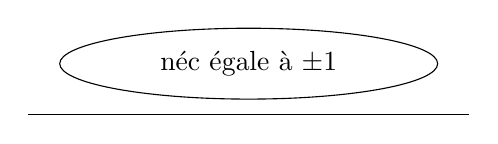
\begin{tikzpicture}
\node (a) at (0,0) {\unsure{néc} \unsure{égale} à $\pm1$};
\draw (0,0) ellipse (2.4 and .45);
\draw (-2.8,-.65)--(2.8,-.65);
\end{tikzpicture}}
\margin{\uline{donc dans l'équation fonctionnelle \unsure{multiplic.} $c$ est un signe}}

Faisons opérer le groupe $\deleted{\unsure{G}}$ $\unsure{\mathbf{Z}|Z}/2\unsure{\mathbf{Z}|Z}$ sur les \inserted{\unsure{gr. mult.}} fonctions rationnelles \inserted{$\ne0$}, par la substitution $t\longmapsto\frac1{qt}$. Alors (pour $c$ donné) la question \unsure{de trouver} $\lambda$

\margin{62}
